%%%%%%%%%%%%%%%%%%%%%%%%%%%%%%%%%%%%%%%%%

%----------------------------------------------------------------------------------------
%	PACKAGES AND OTHER DOCUMENT CONFIGURATIONS
%----------------------------------------------------------------------------------------

\documentclass{article}

\input{C:/Code/TexStudio/templates/structure.tex} % Include the file specifying the document structure and custom commands

%----------------------------------------------------------------------------------------
%	ASSIGNMENT INFORMATION
%----------------------------------------------------------------------------------------

\title{Assignment \#4} % Title of the assignment

\author{Name:Cao Mingming \indent \indent ID:2018311770\\ \texttt{cmm18@mails.tsinghua.edu.cn}} % Author name and email address

\date{Tsinghua University --- \today} % University, school and/or department name(s) and a date

%----------------------------------------------------------------------------------------

\begin{document}

\maketitle % Print the title

%----------------------------------------------------------------------------------------
%	INTRODUCTION
%----------------------------------------------------------------------------------------

\section{Problem 1} % Unnumbered section
Draw the curves similar to Fig. 2.4 for the range of $0<d<2R$ with the parameters that you are
interested in e.g. $R = 15 cm$, $\lambda= 0.37 \mu m$ or $R = 20 cm, \lambda = 0.78\mu $m or $ R=10cm, \lambda=0.532 \mu m$.
\section*{Solution}
According to eqaution 2.21 and 2.22 in textbook we know that,
\begin{equation}
	\begin{array}{l}
		\omega^2=\left(\frac{\lambda R}{n\pi}\right)\sqrt{\frac{d}{2R-d}}\\
		\\
		\omega_{0}^2=\left(\frac{\lambda}{n\pi}\right)\sqrt{\frac{dR}{2}-\frac{d^2}{4}}
	\end{array}
\end{equation}
Choose the parameters as $R = 20 cm, \lambda = 0.78\mu $,we can get the following figure.
\begin{figure}[h]
	\centering
	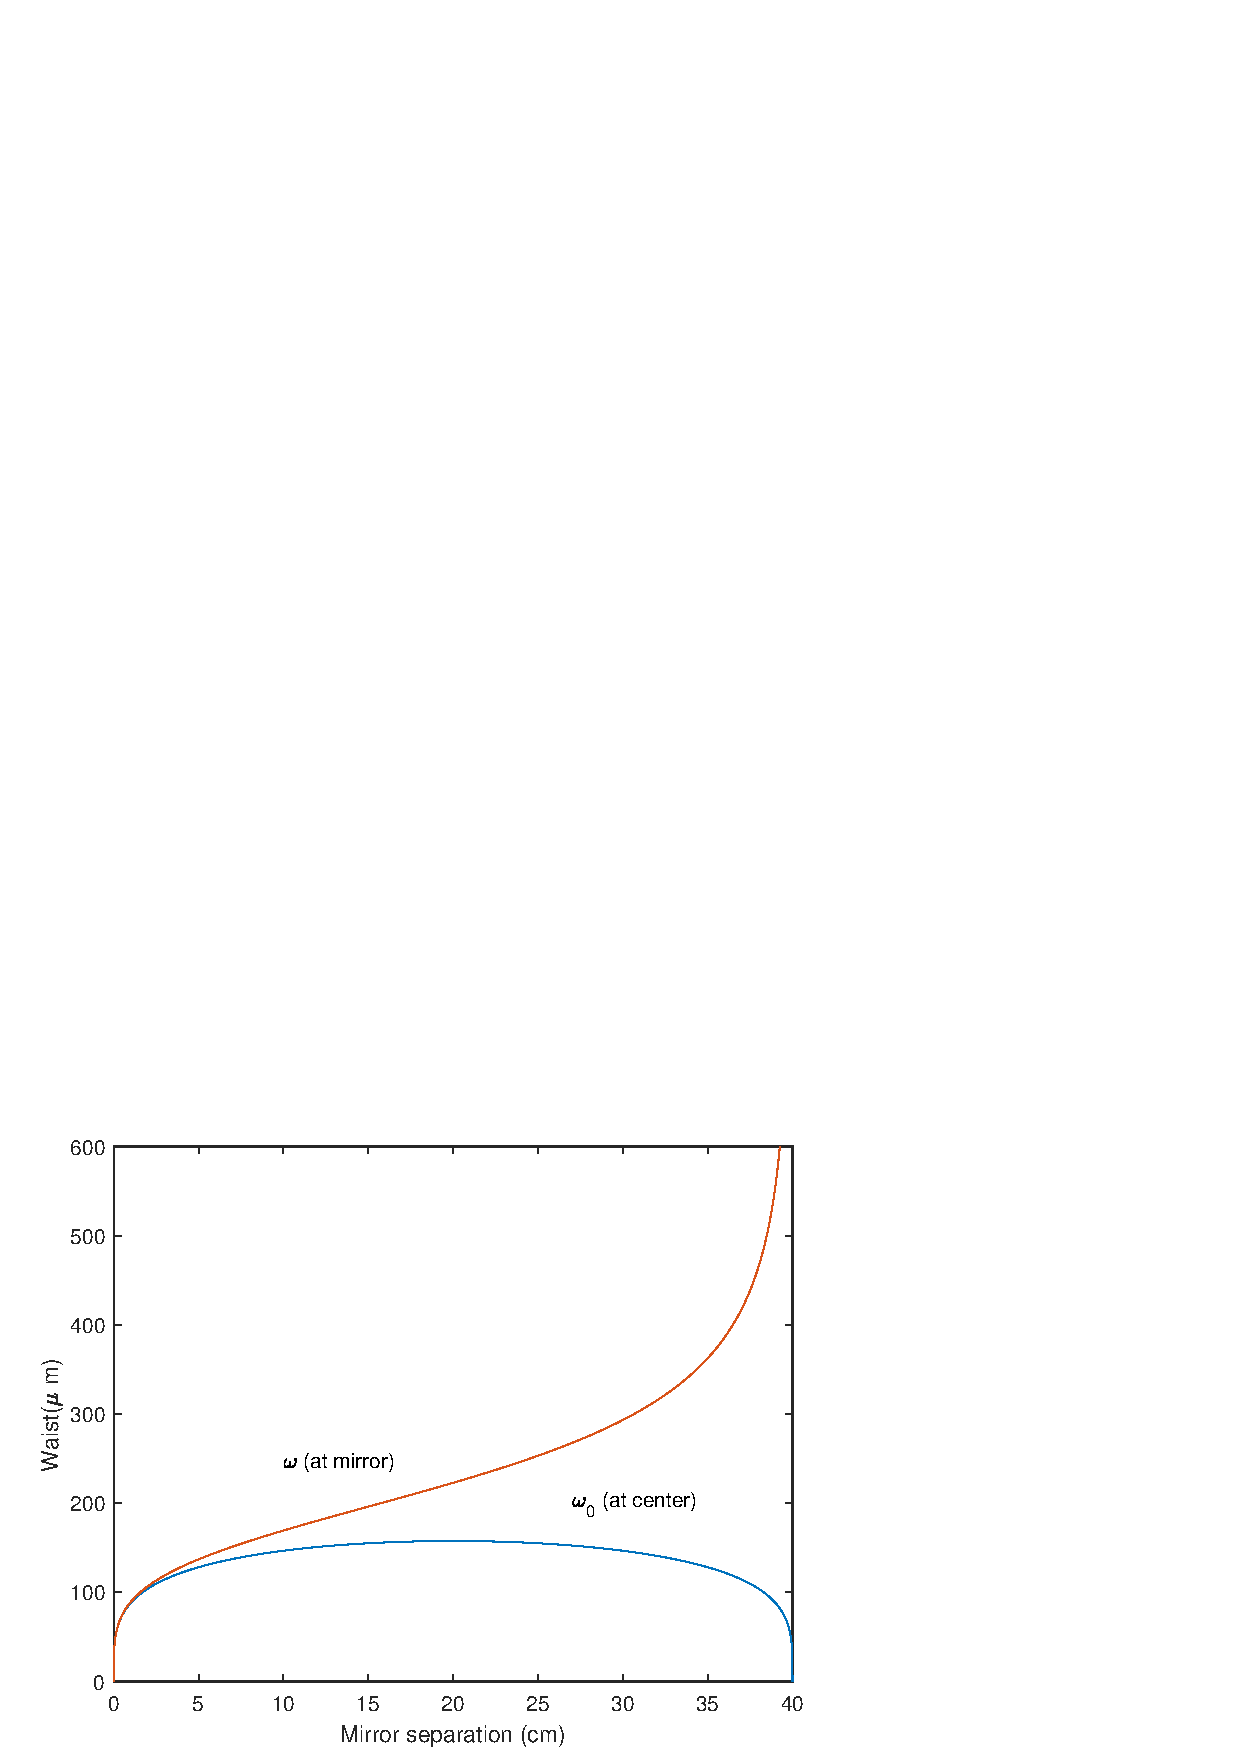
\includegraphics[width=10cm]{f1.pdf}
	\caption{Figure of $\omega $}
\end{figure}

\section{Problem 2}
(a) Find the stability condition in terms of $d_3 , d_1+2d_2$ , and $R$.
(b) Find the small waist within $d_3$ range and the large waist within $d_1$ in terms of $g_1$ ($=1-(d_1+2d_2 )/R$), $g_2$($=1-d_3/R$) and $R$.

\begin{figure}[ht]
	\centering
	\includegraphics[width=10cm]{f2.png}
	\caption{Optical cavity}
\end{figure}

\section*{Solution}
\subsection{a}
According to figure 2 we could get the ABCD matrix as,
\begin{equation}
	\begin{aligned}
	\begin{pmatrix}
	A & B\\
	C & D 
	\end{pmatrix}
	&=\begin{pmatrix}
	1 & 0\\
	-\frac{2}{R} & 1
	\end{pmatrix}
	\begin{pmatrix}
	1 & d_1+2d_2\\
	0 & 1
	\end{pmatrix}
	\begin{pmatrix}
	1 & 0\\
	-\frac{2}{R} & 1
	\end{pmatrix}
	\begin{pmatrix}
	1 & d_3\\
	0 & 1
	\end{pmatrix}\\
	\\
	&=\begin{pmatrix}
	2g_1-1 & R(g_1+g_2-2g_1g_2)\\
	-\frac{4g_1}{R} & 4g_1g_2-2g_1-1
	\end{pmatrix}
	\end{aligned}
\end{equation}
where 
\begin{equation}\label{eq1}
\begin{array}{l}
g_1=1-\frac{d_1+2d_2}{R}\\
\\
g_2=1-\frac{d_3}{R}
\end{array}
\end{equation}
It is the same as what have sloved in two mirror situation  which means we could get the stablity condition as,
\begin{equation}\label{eq2}
|A+D|\leq2\Rightarrow|4g_1g_2-2|\leq2\Rightarrow|0\leq g_1g_2\leq 1
\end{equation}
Take equation \ref{eq1} into equation \ref{eq2} we can get that,
\begin{equation}\label{eq3}
	R \leq d_3 \leq \frac{R(d_1+2d_2)}{d_1+2d_2-R}
\end{equation}
\subsection{b}
By solving the satbility condition we can get that,
\begin{equation}\label{eq4}
	\begin{aligned}
	q_1&=\frac{1}{q}=\frac{D-A}{2B}\pm\frac{1}{2B}\sqrt{(A-D)^2+4BC}\\
	&=\frac{2g_1(g_2-1)}{R(g_1+g_2-2g_1g_2)}\pm i\frac{2\sqrt{g_1g_2(1-g_1g_2)}}{R(g_1+g_2-2g_1g_2)}
	\end{aligned}
\end{equation}
Due to that $q(z)=iz_R+z$ we can derive that,
\begin{equation}\label{key}
	\begin{array}{l}
		z_R=-\frac{Im(q_1)}{|q_1|^2}=\frac{R\sqrt{g_1g_2(1-g_1g_2)}}{2g_1}\\
		\\
		z_1=-\frac{Re(q_1)}{|q_1|^2}=-\frac{R}{2}(g_2-1)=\frac{d_3}{2}
	\end{array}
\end{equation}
where $z_1$ is the location of the left hand curved mirror. From $z_1$ we know that the beam wasit locates at the center of the upper two mirrors. And we can also calculate $q_1$ as,
\begin{equation}\label{eq5}
q_1=\frac{1}{R}-i\frac{\lambda}{n\pi\omega^2}
\end{equation}
By equation \ref{eq5} we can get,
\begin{equation}\label{eq6}
	\begin{array}{l}
	R=z+\frac{z_R^2}{z}\\
	\\
	\omega^2=\frac{\lambda}{n\pi}(z_R+\frac{z^2}{z_R})
	\end{array}
\end{equation}
the size of beam waist comes to minmum when $ z^2 $ comes to minmum($ z^2=0 $). So the largest beam size within $ d_3 $ range locates at the center of two mirrors. And,
\begin{equation}\label{eq7}
	\begin{aligned}
		\omega_0&=\sqrt{\frac{\lambda R}{2n\pi g_1}\sqrt{g_1g_2(1-g_1g_2)}}\\
	\end{aligned}
\end{equation}
Assume that the q parameter at the lower mirror is $q'$, the location of $ q' $ is shown in figure 3.
\begin{figure}[ht]
	\centering
	\includegraphics[width=10cm]{f3.png}
	\caption{Location of q}
\end{figure}
By using ANCD matrix we know when q satisfies the stability condition,
\begin{equation}\label{eq8}
	\begin{array}{l}
	q=\begin{pmatrix}
	1 & 0\\
	-\frac{2}{R} & 1
	\end{pmatrix}
	\begin{pmatrix}
	1 & d_1+2d_2\\
	0 & 1
	\end{pmatrix}
	\begin{pmatrix}
	1 & 0\\
	-\frac{2}{R} & 1
	\end{pmatrix}
	\begin{pmatrix}
	1 & d_3\\
	0 & 1
	\end{pmatrix}q
	\\
	\\
	q'=\begin{pmatrix}
	1 & d_1+2d_2\\
	0 & 1
	\end{pmatrix}
	\begin{pmatrix}
	1 & 0\\
	-\frac{2}{R} & 1
	\end{pmatrix}
	\begin{pmatrix}
	1 & d_3\\
	0 & 1
	\end{pmatrix}q
	\end{array}
\end{equation}
Solving equation \ref{eq8} we can get,
\begin{equation}\label{eq9}
	\begin{aligned}
	q'&=
	\begin{pmatrix}
	1 & 0\\
	-\frac{2}{R} & 1
	\end{pmatrix}^{-1}q\\
	\\
	&=
	\begin{pmatrix}
	1 & 0\\
	\frac{2}{R} & 1
	\end{pmatrix}q
	\end{aligned}
\end{equation}
By equation \ref{eq9} we can get,
\begin{equation}\label{eq10}
	\begin{aligned}
	q_{1}^{'}&=\frac{C+Dq_1}{A+Bq_1}\\
	&=\frac{2}{R}+q1\\
	&=\frac{2g_2(1-g_1)}{R(g_1+g_2-2g_2g_2)}\pm i\frac{2\sqrt{g_1g_2(1-g_1g_2)}}{R(g_1+g_2-2g_1g_2)}
	\end{aligned}
\end{equation}
Use equation 7 we can get $z_{R}^{'}$ and $ \omega_{0}^{'}$ and the location($z_{1}^{'}$) of the $ q' $ .
\begin{equation}\label{eq11}
	\begin{array}{l}
	z_{R}^{'}=\frac{R\sqrt{g_1g_2(1-g_1g_2)}}{2g_2}\\
	\\
	z_{1}^{'}=\frac{R}{2}(g_2-1)=-\frac{d_1+2d_2}{2}\\
	\\
	\omega_{0}^{'}=\frac{\lambda R\sqrt{g_1g_2(1-g_1g_2)}}{2g_2}
	\end{array}
\end{equation}
From equation \ref{eq11} we know that the beam waist locates at the halfway of lower mirror. Use equation 9 we know that,
\begin{equation*}
\omega^2=\frac{\lambda}{n\pi}(z_R+\frac{z^2}{z_R})
\end{equation*}
and z ranges from $[-\frac{d_1}{2},\frac{d_1}{2}]$ so the largest beam size locates at $ z=\pm\frac{d_1}{2} $, which is also the left or right plane lens.
\begin{equation}
	\begin{array}{l}
	\omega_{max}^{'2}=\frac{\lambda}{n\pi}(z_R^{'}+\frac{d_1^2}{4z_R^{'}})\\
	\\
	\omega_{max}^{'}=\sqrt{\frac{\lambda R}{n\pi}\frac{ g_1(1-g_1g_2)+4g_2d_1^2}{2\sqrt{g_1g_2(1-g_1g_2)}}}
	\end{array}
\end{equation}

\section{Problem 3}
Find and draw the size and the Radius of curvature of the beam everywhere inside the cavities with $ R= 6 cm, d_3 = 7 cm, d_1 +2d_2 = 18 cm,  \lambda=0.74 um $. At the curved mirror, how much the radius of curvature is different from R?

\begin{figure}[ht]
	\centering
	\includegraphics[width=10cm]{f4.png}
	\caption{}
\end{figure}


\section*{Solution}
To determine the location of beam, choose the reference plane as the zero point of propagation and ste z as the distance of beam propagates from the reference plane. According to what we have obtained in problem 1 and 2, the beam waist of the upper mirrors locates at $z_1=\frac{d_3}{2}$ and the beam waist of the lower mirrors locate at $z_{1}^{'}=d_2+d_3+\frac{d1}{2}$, using equation 7,9 and 14 we can get the size and radius of curvature while beam propagate btween the mirrors.
\begin{equation}\label{eq12}
	\begin{array}{l}
	\omega(z)=
	\begin{cases}
	\sqrt{\frac{\lambda}{n\pi}(z_R+\frac{(z-z_1)^2)}{z_R}}& 0\leq z \leq d_3\\
	\\
	\sqrt{\frac{\lambda}{n\pi}(z_{R}^{'}+\frac{(z-z_{1}{'})^2}{z_{R}^{'}})} &d_3\leq z \leq d_1+2d_2+d_3
	\end{cases}
	\\
	\\
	R(z)=
	\begin{cases}
	z-z_1+\frac{z_{R}^{2}}{z-z_1}&0\leq z \leq d_3\\
	\\
	z-z_{1}^{'}+\frac{z_{R}^{'2}}{z-z_{1}^{'}} &d_3\leq z \leq d_1+2d_2+d_3
	\end{cases}
	\end{array}
\end{equation}
Finally we can get the figure of beam size and beam curvature as figure 5.And the radius of curvature at the left curved mirror is $r_1=-3.6429cm $, at the right is $r_2=3.6429cm$
\begin{figure}
	\begin{minipage}[t]{0.5\linewidth}
	\centering
	\includegraphics[width=7cm]{f31.eps}
	\caption{Figure of beam size}
	\label{fig:side:a}
	\end{minipage}%
	\begin{minipage}[t]{0.5\linewidth}
	\centering
	\includegraphics[width=7cm]{f32.eps}
	\caption{Figure of beam Radius}
	\label{fig:side:b}
	\end{minipage}
\end{figure}


\end{document}